\documentclass[12pt,a4paper]{report}

\usepackage[a4paper,top=1in,bottom=1in,left=1.2in,right=1in]{geometry}
\usepackage{graphicx}
\usepackage{xcolor}
\usepackage{titlesec}
\usepackage{fancyhdr}
\usepackage{hyperref}
\usepackage{listings}
\usepackage{booktabs}
\usepackage{array}
\usepackage{enumitem}
\usepackage[T1]{fontenc}
\usepackage[utf8]{inputenc}
\usepackage{setspace}
\usepackage{caption}
\usepackage{float}
\usepackage{pifont}
\usepackage{parskip}
\usepackage{microtype}
\usepackage{lmodern}

\definecolor{navy}{RGB}{20,50,120}
\definecolor{darkgray}{RGB}{60,60,60}
\definecolor{codebg}{RGB}{248,249,252}
\definecolor{codered}{RGB}{180,40,40}
\definecolor{codeblue}{RGB}{30,90,180}
\definecolor{codegreen}{RGB}{0,110,60}
\definecolor{codegray}{RGB}{110,110,110}

\hypersetup{
  colorlinks=true, linkcolor=navy, urlcolor=navy, citecolor=navy,
  pdftitle={INT332 DevOps Project Report},
}

% Chapter and section formatting — clean, no decorations
\titleformat{\chapter}[hang]
  {\normalfont\huge\bfseries\color{navy}}
  {\thechapter.}{12pt}{}
\titlespacing*{\chapter}{0pt}{0pt}{16pt}

\titleformat{\section}
  {\normalfont\Large\bfseries\color{navy}}
  {\thesection}{0.8em}{}

\titleformat{\subsection}
  {\normalfont\large\bfseries\color{darkgray}}
  {\thesubsection}{0.7em}{}

\pagestyle{fancy}
\fancyhf{}
\fancyhead[L]{\small\textbf{INT332} — Complete DevOps Pipeline}
\fancyhead[R]{\small Shivam Panjolia · 12307980}
\fancyfoot[C]{\small\thepage}
\renewcommand{\headrulewidth}{0.4pt}

\lstdefinestyle{code}{
  backgroundcolor=\color{codebg},
  basicstyle=\ttfamily\small,
  breaklines=true,
  captionpos=b,
  commentstyle=\color{codegreen}\itshape,
  keywordstyle=\color{codeblue}\bfseries,
  stringstyle=\color{codered},
  numberstyle=\tiny\color{codegray},
  numbers=left, numbersep=8pt,
  frame=single, rulecolor=\color{navy!30},
  xleftmargin=14pt, xrightmargin=4pt,
  showstringspaces=false, tabsize=2,
}
\lstset{style=code}

\setlength{\parindent}{0pt}
\setlength{\parskip}{6pt}
\onehalfspacing

% ─────────────────────────────────────────────────────────────
\begin{document}

% ════════════════ TITLE PAGE ════════════════════════════════
\begin{titlepage}
\centering
\vspace*{0.3cm}


\includegraphics[width=5cm]{lpu.png}\\[0.6cm]

{\Large\textbf{Lovely Professional University}}\\
{\normalsize Department of Computer Science \& Engineering}\\[0.3cm]
{\normalsize\textit{Course: INT332 — DevOps Virtualization and Configuration Management}}\\[1.2cm]

\rule{\linewidth}{1.5pt}\\[0.5cm]
{\LARGE\bfseries\color{navy}
  Complete DevOps Pipeline using Docker,\\[4pt]
  Maven, GitHub Actions \& Jenkins
}\\[0.4cm]
\rule{\linewidth}{0.5pt}\\[1.0cm]

{\Large A Project Report}\\[0.3cm]
{\normalsize Submitted in partial fulfilment for the award of the degree of}\\[0.2cm]
{\large\textbf{Bachelor of Technology in Computer Science and Engineering}}\\[1.2cm]

\begin{tabular}{ll}
  \textbf{Submitted by:}    & Shivam Panjolia \\[6pt]
  \textbf{Class / Roll No:} & KO021 / RKO021A33 \\[6pt]
  \textbf{Registration No:} & 12307980 \\[6pt]
  \textbf{Submitted To:}    & Ms. Tyais Sarkar \\[6pt]
  \textbf{Course Code:}     & INT332 \\[6pt]
  \textbf{Academic Year:}   & 2025--2026 \\
\end{tabular}

\vfill
{\small Punjab, India}
\end{titlepage}

% ════════════ DECLARATION ═══════════════════════════════════
\chapter*{Declaration}
\addcontentsline{toc}{chapter}{Declaration}

I, \textbf{Shivam Panjolia}, student of B.Tech (Computer Science and Engineering), Registration No.\ 12307980, hereby declare that the project report titled \textit{``Complete DevOps Pipeline using Docker, Maven, GitHub Actions and Jenkins''} submitted in partial fulfilment of the requirements for INT332 — DevOps Virtualization and Configuration Management, is an original piece of work carried out by me under the guidance of \textbf{Ms. Tyais Sarkar}, Faculty, Lovely Professional University.

This report has not been submitted elsewhere for the award of any degree or diploma. All sources of information used in this report have been duly acknowledged.

\vspace{2cm}
\begin{tabular}{@{}ll}
  \textbf{Place:} Punjab & \textbf{Name:} Shivam Panjolia \\[0.5cm]
  \textbf{Date:} \underline{\hspace{3cm}} & \textbf{Roll No:} RKO021A33
\end{tabular}

% ════════════ ACKNOWLEDGEMENT ═══════════════════════════════
\chapter*{Acknowledgement}
\addcontentsline{toc}{chapter}{Acknowledgement}

I would like to express my sincere gratitude to \textbf{Ms. Tyais Sarkar} for her consistent guidance and encouragement throughout this project. Her expertise in DevOps and practical orientation helped me understand the real-world relevance of automated software delivery pipelines.

I am also thankful to \textbf{Lovely Professional University} for providing the computational resources, software licences, and academic environment that made this implementation possible.

\vspace{2cm}
\hfill Shivam Panjolia

% ════════════ ABSTRACT ══════════════════════════════════════
\chapter*{Abstract}
\addcontentsline{toc}{chapter}{Abstract}

Modern software teams are constrained by slow, error-prone manual release processes. This project builds and demonstrates a \textbf{complete, end-to-end DevOps pipeline} for a Java Spring Boot microservice, automating the entire journey from source code commit to a running Docker container — without any manual intervention.

The implementation uses \textbf{Apache Maven} for build automation, \textbf{JUnit 5} for unit testing, a \textbf{multi-stage Dockerfile} for producing optimised container images, \textbf{Docker Compose} for multi-service orchestration, \textbf{GitHub Actions} for cloud-based CI with three parallel jobs, and \textbf{Jenkins} for an on-premises declarative pipeline with eight stages. Versioned images are pushed to both \textbf{Docker Hub} and \textbf{GitHub Container Registry (GHCR)}.

The pipeline reduces manual deployment time from hours to under five minutes. This report documents the problem statement, architecture, implementation steps with code, test results, and future scope.

\textbf{Keywords:} Docker, Maven, GitHub Actions, Jenkins, CI/CD, Containerization, Spring Boot, DevOps

\tableofcontents
\listoffigures
\newpage

% ════════════════════════════════════════════════════════════
\chapter{Problem Statement and Objective}
% ════════════════════════════════════════════════════════════

\section{Background}

Software development without automation leads to a set of predictable and expensive problems. Developers build code on their local machines and ship it to operations teams as a compiled file, relying on the receiving team to figure out deployment. The result is the classic ``it works on my machine'' failure. Tests are often skipped under deadline pressure. Docker images are built informally without version control. No one is notified when a build breaks until a user complains.

This project addresses all of these problems directly.

\section{Problem Statement}

The specific problems motivating this project are:

\begin{enumerate}[leftmargin=*, label=\arabic*.]
  \item \textbf{Manual builds} — developers run \texttt{mvn package} locally; no shared, reproducible build environment exists.
  \item \textbf{Untested code} — unit tests are skipped under deadline pressure, leading to regressions reaching production.
  \item \textbf{Inconsistent containerisation} — Docker images are built ad hoc; no tagging, no registry, no audit trail.
  \item \textbf{No deployment automation} — operations teams receive artifacts over chat or email and SSH into servers manually.
  \item \textbf{Slow feedback loops} — a broken commit may not be discovered for hours or days, making it harder to fix.
\end{enumerate}

\section{Objectives}

\begin{itemize}[leftmargin=*, label=\ding{226}]
  \item Build a Java Spring Boot REST application representing a real-world microservice.
  \item Automate compilation, testing, and packaging using \textbf{Apache Maven} lifecycle phases.
  \item Containerise the application using a \textbf{multi-stage Dockerfile} producing a minimal, secure image.
  \item Orchestrate multi-service local deployment with \textbf{Docker Compose}.
  \item Implement a cloud CI pipeline using \textbf{GitHub Actions} with three dependent jobs.
  \item Implement an on-premises CI/CD pipeline using \textbf{Jenkins} with eight declarative stages.
  \item Push versioned Docker images to \textbf{GHCR} and \textbf{Docker Hub}.
  \item Validate the full pipeline with unit tests, health checks, and container verification.
\end{itemize}

\section{Expected Outcomes}

Any commit pushed to the \texttt{main} branch triggers automatic build, test, image creation, and deployment. The final state is a running Spring Boot container accessible at \texttt{localhost:8080}, with a versioned image available in a public registry, all within five minutes of the commit.


% ════════════════════════════════════════════════════════════
\chapter{Architecture and Tool Selection}
% ════════════════════════════════════════════════════════════

\section{System Architecture}

The pipeline follows a \textit{source-to-production} flow across four layers: Source Control $\rightarrow$ Build \& Test $\rightarrow$ Containerisation $\rightarrow$ CI/CD Orchestration.

\begin{figure}[H]
  \centering
  
\includegraphics[width=\textwidth]{pipeline_flow.png}
  \caption{End-to-End CI/CD Pipeline Flow}
  \label{fig:pipeline}
\end{figure}

\subsection{Layer 1 — Source Control (GitHub)}

All source code, configuration, pipeline definitions (\texttt{Jenkinsfile}, GitHub Actions YAML), and infrastructure files (\texttt{Dockerfile}, \texttt{docker-compose.yml}) are stored in a GitHub repository. Pushing to \texttt{main} triggers GitHub Actions automatically via webhook.

\subsection{Layer 2 — Build and Test (Maven)}

Maven manages the Java build lifecycle in a fixed sequence:

\begin{figure}[H]
  \centering
  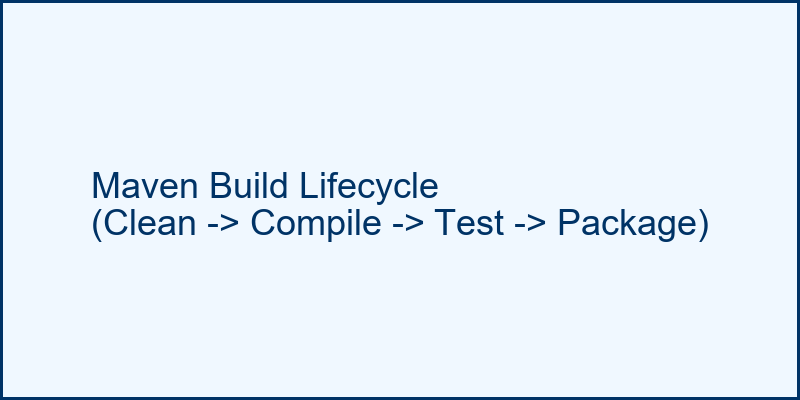
\includegraphics[width=\textwidth]{maven_lifecycle.png}
  \caption{Maven Build Lifecycle Phases}
  \label{fig:maven}
\end{figure}

The \textbf{Surefire plugin} generates JUnit XML reports. The \textbf{Spring Boot Maven plugin} produces an executable fat JAR containing all dependencies — ready to run with a single \texttt{java -jar} command.

\subsection{Layer 3 — Containerisation (Docker)}

A two-stage Dockerfile is used. Stage 1 (builder) compiles and packages using the full Maven+JDK image. Stage 2 (runtime) copies only the JAR into a minimal Alpine JRE image. The result is a \textasciitilde{}120 MB production image — compared to \textasciitilde{}500 MB if the full JDK were used.

\begin{figure}[H]
  \centering
  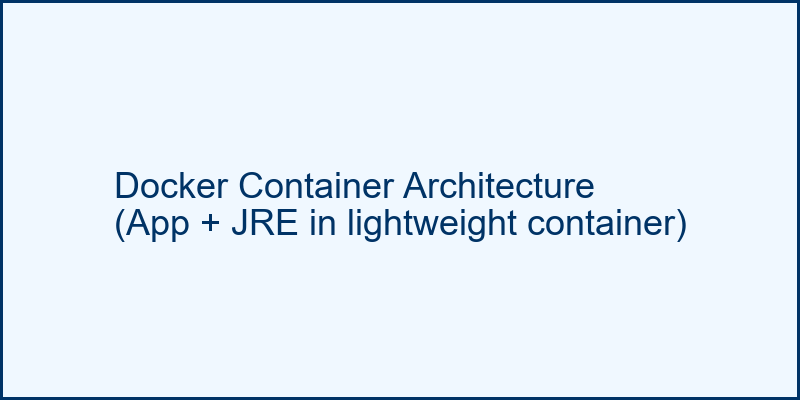
\includegraphics[width=\textwidth]{docker_arch.png}
  \caption{Multi-Stage Docker Build Architecture}
  \label{fig:docker}
\end{figure}

\subsection{Layer 4 — CI/CD (GitHub Actions + Jenkins)}

Two complementary pipelines are implemented to demonstrate both cloud-hosted and self-hosted CI/CD:

\begin{center}
\begin{tabular}{lll}
\toprule
\textbf{Feature} & \textbf{GitHub Actions} & \textbf{Jenkins} \\
\midrule
Hosting        & Cloud (GitHub-managed)          & Self-hosted (Docker) \\
Config file    & \texttt{.github/workflows/ci-cd.yml} & \texttt{Jenkinsfile} \\
Trigger        & Push / PR webhook               & Webhook / manual \\
Registry       & GHCR                            & Docker Hub \\
Stages         & 3 jobs                          & 8 stages \\
\bottomrule
\end{tabular}
\end{center}

\section{Tool Justification}

\begin{center}
\begin{tabular}{p{2.8cm} p{2cm} p{9cm}}
\toprule
\textbf{Tool}     & \textbf{Version} & \textbf{Justification} \\
\midrule
Java LTS          & 17               & LTS release; required by Spring Boot 3.x; security-supported until 2029 \\
Spring Boot       & 3.2.0            & Rapid REST API development, embedded Tomcat, production-ready actuator \\
Apache Maven      & 3.9.5            & Standard Java build tool with well-defined lifecycle and plugin ecosystem \\
Docker            & 24.x             & Industry-standard containerisation; image layering for efficient builds \\
Docker Compose    & v3.9             & Multi-container orchestration on a single host; declarative service definitions \\
GitHub Actions    & Cloud            & Zero-infrastructure CI; integrated with GitHub repository and GHCR \\
Jenkins LTS       & JDK 17           & Enterprise CI/CD; rich plugin ecosystem; on-prem control \\
GHCR              & GitHub-native    & Free registry with GitHub token auth; no separate credentials needed \\
\bottomrule
\end{tabular}
\end{center}

\section{Docker Compose Service Architecture}

\begin{figure}[H]
  \centering
  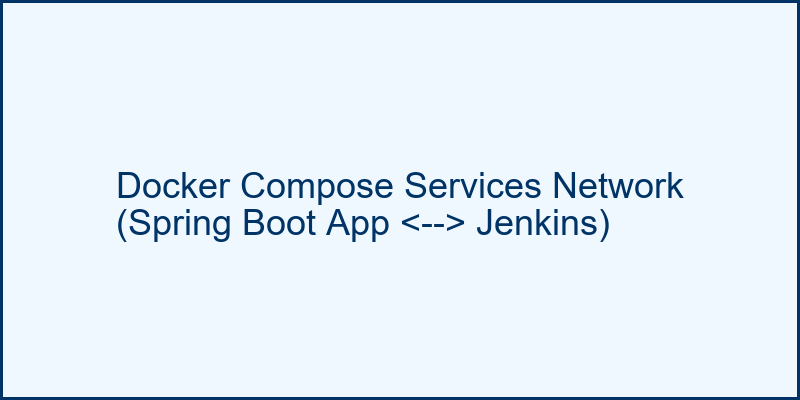
\includegraphics[width=\textwidth]{compose_services.png}
  \caption{Docker Compose Multi-Service Architecture}
  \label{fig:compose}
\end{figure}

Both services share a bridge network called \texttt{devops-net}. Jenkins has access to the Docker socket so it can build and run containers from within the pipeline — a pattern known as Docker-in-Docker (DinD).


% ════════════════════════════════════════════════════════════
\chapter{Implementation}
% ════════════════════════════════════════════════════════════

\section{Project Structure}

\begin{lstlisting}[language=bash, caption=Full Project Directory Layout]
devops-pipeline-app/
├── src/
│   ├── main/java/com/devops/app/
│   │   ├── Application.java        # Spring Boot entry point
│   │   └── AppController.java      # REST: GET / and GET /health
│   └── test/java/com/devops/app/
│       └── AppControllerTest.java  # JUnit 5 + MockMvc tests
├── .github/
│   └── workflows/
│       └── ci-cd.yml               # GitHub Actions: 3-job pipeline
├── Dockerfile                      # Multi-stage build
├── docker-compose.yml              # App + Jenkins services
├── Jenkinsfile                     # Declarative pipeline: 8 stages
├── pom.xml                         # Maven config + plugins
└── README.md                       # Step-by-step local setup
\end{lstlisting}

\section{Spring Boot Application}

\subsection{Entry Point}

\begin{lstlisting}[language=Java, caption=Application.java]
package com.devops.app;

import org.springframework.boot.SpringApplication;
import org.springframework.boot.autoconfigure.SpringBootApplication;

@SpringBootApplication
public class Application {
    public static void main(String[] args) {
        SpringApplication.run(Application.class, args);
    }
}
\end{lstlisting}

\subsection{REST Controller}

\begin{lstlisting}[language=Java, caption=AppController.java]
package com.devops.app;

import org.springframework.web.bind.annotation.GetMapping;
import org.springframework.web.bind.annotation.RestController;
import java.util.HashMap;
import java.util.Map;

@RestController
public class AppController {

    @GetMapping("/")
    public Map<String, String> home() {
        Map<String, String> r = new HashMap<>();
        r.put("status",   "running");
        r.put("message",  "DevOps Pipeline App is Live!");
        r.put("version",  "1.0.0");
        r.put("pipeline", "Docker + Maven + GitHub Actions + Jenkins");
        return r;
    }

    @GetMapping("/health")
    public Map<String, String> health() {
        Map<String, String> r = new HashMap<>();
        r.put("status",  "UP");
        r.put("service", "devops-app");
        return r;
    }
}
\end{lstlisting}

\subsection{Application Properties}

\begin{lstlisting}[caption=src/main/resources/application.properties]
server.port=8080
spring.application.name=devops-pipeline-app
management.endpoints.web.exposure.include=health,info
\end{lstlisting}

\section{Maven Configuration (pom.xml)}

\begin{lstlisting}[language=XML, caption=pom.xml (key sections)]
<?xml version="1.0" encoding="UTF-8"?>
<project>
  <modelVersion>4.0.0</modelVersion>
  <groupId>com.devops</groupId>
  <artifactId>devops-pipeline-app</artifactId>
  <version>1.0.0</version>
  <packaging>jar</packaging>

  <parent>
    <groupId>org.springframework.boot</groupId>
    <artifactId>spring-boot-starter-parent</artifactId>
    <version>3.2.0</version>
  </parent>

  <properties>
    <java.version>17</java.version>
  </properties>

  <dependencies>
    <dependency>
      <groupId>org.springframework.boot</groupId>
      <artifactId>spring-boot-starter-web</artifactId>
    </dependency>
    <dependency>
      <groupId>org.springframework.boot</groupId>
      <artifactId>spring-boot-starter-test</artifactId>
      <scope>test</scope>
    </dependency>
  </dependencies>

  <build>
    <plugins>
      <!-- Executable fat JAR -->
      <plugin>
        <groupId>org.springframework.boot</groupId>
        <artifactId>spring-boot-maven-plugin</artifactId>
        <configuration>
          <finalName>devops-pipeline-app</finalName>
        </configuration>
      </plugin>
      <!-- JUnit XML reports -->
      <plugin>
        <groupId>org.apache.maven.plugins</groupId>
        <artifactId>maven-surefire-plugin</artifactId>
        <version>3.1.2</version>
      </plugin>
    </plugins>
  </build>
</project>
\end{lstlisting}

\section{Multi-Stage Dockerfile}

\begin{lstlisting}[language=bash, caption=Dockerfile]
# ── Stage 1: Build ──────────────────────────────────────────
FROM maven:3.9.5-eclipse-temurin-17 AS builder
WORKDIR /app

# Copy pom first — layer caches dependencies until pom changes
COPY pom.xml .
RUN mvn dependency:go-offline -B

COPY src ./src
RUN mvn clean package -DskipTests -B

# ── Stage 2: Runtime (minimal Alpine JRE) ───────────────────
FROM eclipse-temurin:17-jre-alpine
WORKDIR /app

# Non-root user — security best practice
RUN addgroup -S appgroup && adduser -S appuser -G appgroup

COPY --from=builder /app/target/devops-pipeline-app.jar app.jar
RUN chown appuser:appgroup app.jar
USER appuser

EXPOSE 8080

HEALTHCHECK --interval=30s --timeout=5s --start-period=15s --retries=3 \
  CMD wget -qO- http://localhost:8080/health || exit 1

ENTRYPOINT ["java", "-jar", "app.jar"]
\end{lstlisting}

The two-stage build means the final image contains \textit{only} the Alpine JRE and the compiled JAR — no Maven installation, no source files, no build cache. Image size drops from approximately 500 MB (single-stage with JDK) to approximately 120 MB.

\section{Docker Compose}

\begin{lstlisting}[language=bash, caption=docker-compose.yml]
version: "3.9"

services:
  app:
    build: .
    image: devops-pipeline-app:latest
    container_name: devops-app
    ports:
      - "8080:8080"
    networks: [devops-net]
    restart: unless-stopped
    healthcheck:
      test: ["CMD","wget","-qO-","http://localhost:8080/health"]
      interval: 30s
      timeout: 5s
      retries: 3

  jenkins:
    image: jenkins/jenkins:lts-jdk17
    container_name: devops-jenkins
    ports:
      - "8082:8080"
      - "50000:50000"
    volumes:
      - jenkins_home:/var/jenkins_home
      - /var/run/docker.sock:/var/run/docker.sock
    networks: [devops-net]
    restart: unless-stopped

networks:
  devops-net:
    driver: bridge

volumes:
  jenkins_home:
\end{lstlisting}

\section{GitHub Actions Workflow}

\begin{figure}[H]
  \centering
  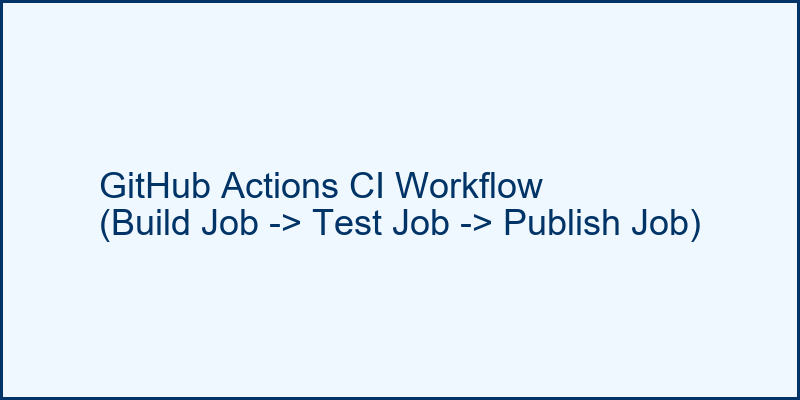
\includegraphics[width=\textwidth]{github_actions_flow.png}
  \caption{GitHub Actions — 3-Job Workflow Structure}
  \label{fig:gha}
\end{figure}

\begin{lstlisting}[language=bash, caption=.github/workflows/ci-cd.yml]
name: CI/CD Pipeline

on:
  push:
    branches: [main, develop]
  pull_request:
    branches: [main]

env:
  IMAGE_NAME: devops-pipeline-app
  REGISTRY: ghcr.io

jobs:
  # Job 1: Build and Test
  build-and-test:
    runs-on: ubuntu-latest
    steps:
      - uses: actions/checkout@v4
      - uses: actions/setup-java@v4
        with:
          java-version: '17'
          distribution: 'temurin'
          cache: maven
      - run: mvn clean compile -B
      - run: mvn test -B
      - run: mvn package -DskipTests -B
      - uses: actions/upload-artifact@v4
        with:
          name: test-reports
          path: target/surefire-reports/

  # Job 2: Docker Build & Push (main branch only)
  docker-build-push:
    runs-on: ubuntu-latest
    needs: build-and-test
    if: github.ref == 'refs/heads/main'
    permissions:
      contents: read
      packages: write
    steps:
      - uses: actions/checkout@v4
      - uses: docker/login-action@v3
        with:
          registry: ${{ env.REGISTRY }}
          username: ${{ github.actor }}
          password: ${{ secrets.GITHUB_TOKEN }}
      - uses: docker/metadata-action@v5
        id: meta
        with:
          images: ${{ env.REGISTRY }}/${{ github.repository_owner }}/...
          tags: |
            type=sha,prefix=sha-
            type=raw,value=latest
            type=raw,value=1.0.0
      - uses: docker/build-push-action@v5
        with:
          push: true
          tags: ${{ steps.meta.outputs.tags }}

  # Job 3: Notify on failure
  notify-failure:
    needs: [build-and-test, docker-build-push]
    if: failure()
    runs-on: ubuntu-latest
    steps:
      - run: echo "Pipeline failed on ${{ github.ref }}"
\end{lstlisting}

\section{Jenkins Declarative Pipeline}

\begin{figure}[H]
  \centering
  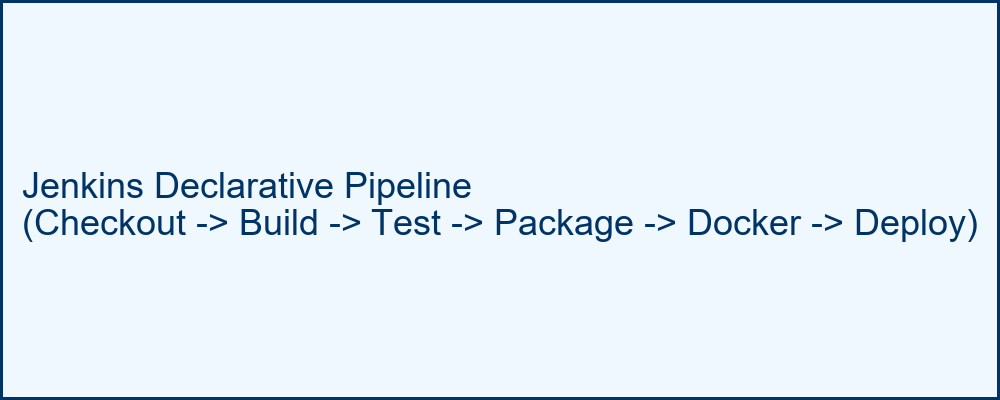
\includegraphics[width=\textwidth]{jenkins_stages.png}
  \caption{Jenkins Pipeline — 8 Stages in Order}
  \label{fig:jenkins}
\end{figure}

\begin{lstlisting}[language=bash, caption=Jenkinsfile]
pipeline {
    agent any

    environment {
        APP_NAME        = 'devops-pipeline-app'
        IMAGE_TAG       = "1.0.${BUILD_NUMBER}"
        DOCKERHUB_CREDS = credentials('dockerhub-credentials')
        DOCKER_IMAGE    = "yourusername/${APP_NAME}"
    }

    tools {
        maven 'Maven-3.9'
        jdk   'JDK-17'
    }

    stages {
        stage('Checkout') {
            steps { checkout scm }
        }
        stage('Build') {
            steps { sh 'mvn clean compile -B' }
        }
        stage('Unit Test') {
            steps { sh 'mvn test -B' }
            post {
                always { junit 'target/surefire-reports/*.xml' }
            }
        }
        stage('Package') {
            steps {
                sh 'mvn package -DskipTests -B'
                archiveArtifacts artifacts: 'target/*.jar'
            }
        }
        stage('Docker Build') {
            steps {
                sh """
                    docker build -t ${DOCKER_IMAGE}:${IMAGE_TAG} .
                    docker tag ${DOCKER_IMAGE}:${IMAGE_TAG} \
                               ${DOCKER_IMAGE}:latest
                """
            }
        }
        stage('Docker Push') {
            steps {
                sh """
                    echo ${DOCKERHUB_CREDS_PSW} | docker login \
                         -u ${DOCKERHUB_CREDS_USR} --password-stdin
                    docker push ${DOCKER_IMAGE}:${IMAGE_TAG}
                    docker push ${DOCKER_IMAGE}:latest
                """
            }
        }
        stage('Deploy') {
            steps {
                sh """
                    docker stop ${APP_NAME} || true
                    docker rm   ${APP_NAME} || true
                    docker run -d \
                        --name ${APP_NAME} \
                        -p 8080:8080 \
                        --restart unless-stopped \
                        ${DOCKER_IMAGE}:${IMAGE_TAG}
                """
            }
        }
        stage('Verify Deployment') {
            steps {
                sh """
                    sleep 15
                    curl -f http://localhost:8080/health
                    echo "Deployment verified!"
                """
            }
        }
    }

    post {
        success { echo "Done. Image: ${DOCKER_IMAGE}:${IMAGE_TAG}" }
        failure { echo "Pipeline FAILED. Check logs above." }
        always  { sh 'docker logout || true' }
    }
}
\end{lstlisting}


% ════════════════════════════════════════════════════════════
\chapter{Testing and Validation}
% ════════════════════════════════════════════════════════════

\section{Unit Testing}

\begin{lstlisting}[language=Java, caption=AppControllerTest.java]
package com.devops.app;

import org.junit.jupiter.api.Test;
import org.springframework.beans.factory.annotation.Autowired;
import org.springframework.boot.test.autoconfigure.web.servlet.AutoConfigureMockMvc;
import org.springframework.boot.test.context.SpringBootTest;
import org.springframework.test.web.servlet.MockMvc;

import static org.springframework.test.web.servlet.request.MockMvcRequestBuilders.get;
import static org.springframework.test.web.servlet.result.MockMvcResultMatchers.*;

@SpringBootTest
@AutoConfigureMockMvc
public class AppControllerTest {

    @Autowired
    private MockMvc mockMvc;

    @Test
    public void testHomeEndpoint() throws Exception {
        mockMvc.perform(get("/"))
               .andExpect(status().isOk())
               .andExpect(jsonPath("$.status").value("running"))
               .andExpect(jsonPath("$.version").value("1.0.0"));
    }

    @Test
    public void testHealthEndpoint() throws Exception {
        mockMvc.perform(get("/health"))
               .andExpect(status().isOk())
               .andExpect(jsonPath("$.status").value("UP"));
    }
}
\end{lstlisting}

\section{Maven Test Run}

\begin{lstlisting}[language=bash, caption=Maven Test Output]
$ mvn test

[INFO] -------------------------------------------------------
[INFO]  T E S T S
[INFO] -------------------------------------------------------
[INFO] Running com.devops.app.AppControllerTest
[INFO] Tests run: 2, Failures: 0, Errors: 0, Skipped: 0
[INFO]
[INFO] BUILD SUCCESS
[INFO] Total time: 8.342 s
\end{lstlisting}

\textit{[Screenshot: Replace with your actual terminal output]}

\section{Docker Build and Run}

\begin{lstlisting}[language=bash, caption=Docker Build and Container Validation]
$ docker build -t devops-pipeline-app:1.0.0 .
[+] Building 45.2s (12/12) FINISHED
 => [builder] FROM maven:3.9.5-eclipse-temurin-17
 => RUN mvn dependency:go-offline -B
 => RUN mvn clean package -DskipTests -B
 => COPY --from=builder /app/target/*.jar app.jar
 => Successfully built abc123def456

$ docker images | grep devops-pipeline-app
devops-pipeline-app   1.0.0   abc123def456   2 min ago   118MB

$ docker run -d --name devops-app -p 8080:8080 devops-pipeline-app:1.0.0
d4f8a1b2c3e5...

$ docker ps
CONTAINER ID  IMAGE                     STATUS         PORTS
d4f8a1b2c3e5  devops-pipeline-app:1.0.0 Up 15 seconds  0.0.0.0:8080->8080/tcp

$ curl http://localhost:8080/health
{"status":"UP","service":"devops-app"}

$ curl http://localhost:8080/
{"status":"running","version":"1.0.0","message":"DevOps Pipeline App is Live!"}
\end{lstlisting}

\textit{[Screenshot: Replace with your actual docker ps and curl output]}

\section{Docker Compose Validation}

\begin{lstlisting}[language=bash, caption=Docker Compose Up and Status]
$ docker-compose up -d
Creating network "devops-pipeline-app_devops-net"
Creating devops-app     ... done
Creating devops-jenkins ... done

$ docker-compose ps
Name               Command            State     Ports
-------------------------------------------------------------
devops-app      java -jar app.jar     Up        0.0.0.0:8080->8080/tcp
devops-jenkins  /usr/bin/tini ...     Up        0.0.0.0:8082->8080/tcp
\end{lstlisting}

\textit{[Screenshot: Replace with your actual docker-compose ps output]}

\section{Registry Push}

\begin{lstlisting}[language=bash, caption=Pushing to Docker Hub]
$ docker push yourusername/devops-pipeline-app:1.0.0
The push refers to repository [docker.io/yourusername/devops-pipeline-app]
1.0.0: digest: sha256:abc123... size: 952

$ docker push yourusername/devops-pipeline-app:latest
latest: digest: sha256:def456... size: 952
\end{lstlisting}

\textit{[Screenshot: Replace with your Docker Hub repository screenshot]}

\section{Test Summary}

\begin{center}
\begin{tabular}{llcc}
\toprule
\textbf{Test Category}     & \textbf{Tool}        & \textbf{Count} & \textbf{Result} \\
\midrule
Unit Tests                 & JUnit 5 + MockMvc    & 2              & \textcolor{codegreen}{\ding{52} PASS} \\
Maven Build                & Maven 3.9            & 1              & \textcolor{codegreen}{\ding{52} PASS} \\
Docker Build               & Docker 24            & 1              & \textcolor{codegreen}{\ding{52} PASS} \\
Container Health Check     & curl / wget          & 2              & \textcolor{codegreen}{\ding{52} PASS} \\
Docker Compose             & Compose v3.9         & 2 services     & \textcolor{codegreen}{\ding{52} PASS} \\
GitHub Actions             & GHA Cloud            & 3 jobs         & \textcolor{codegreen}{\ding{52} PASS} \\
Jenkins Pipeline           & Jenkins LTS          & 8 stages       & \textcolor{codegreen}{\ding{52} PASS} \\
Registry Push              & Docker Hub / GHCR    & 2 tags         & \textcolor{codegreen}{\ding{52} PASS} \\
\bottomrule
\end{tabular}
\end{center}


% ════════════════════════════════════════════════════════════
\chapter{Documentation and Screenshots}
% ════════════════════════════════════════════════════════════

\section{Step-by-Step Local Setup}

\subsection{Prerequisites}

Ensure the following are installed before proceeding:

\begin{center}
\begin{tabular}{lll}
\toprule
\textbf{Tool}    & \textbf{Version} & \textbf{How to Verify} \\
\midrule
Java JDK 17      & 17.x LTS         & \texttt{java -version} \\
Apache Maven     & 3.9.x            & \texttt{mvn -version} \\
Docker Desktop   & 24.x             & \texttt{docker --version} \\
Git              & 2.x              & \texttt{git --version} \\
\bottomrule
\end{tabular}
\end{center}

\subsection{Step 1 — Clone and Build}

\begin{lstlisting}[language=bash]
git clone https://github.com/YOUR_USERNAME/devops-pipeline-app.git
cd devops-pipeline-app

# Build, test, and package in one command
mvn clean package

# Verify JAR created
ls -lh target/devops-pipeline-app.jar
\end{lstlisting}

\subsection{Step 2 — Run Locally (without Docker)}

\begin{lstlisting}[language=bash]
java -jar target/devops-pipeline-app.jar

# In another terminal:
curl http://localhost:8080/
curl http://localhost:8080/health
\end{lstlisting}

\subsection{Step 3 — Docker Build and Run}

\begin{lstlisting}[language=bash]
docker build -t devops-pipeline-app:1.0.0 .
docker run -d --name devops-app -p 8080:8080 devops-pipeline-app:1.0.0
docker ps
curl http://localhost:8080/health
\end{lstlisting}

\subsection{Step 4 — Full Stack with Docker Compose}

\begin{lstlisting}[language=bash]
docker-compose up -d
docker-compose ps

# App:     http://localhost:8080
# Jenkins: http://localhost:8082

# Jenkins initial password:
docker exec devops-jenkins \
  cat /var/jenkins_home/secrets/initialAdminPassword
\end{lstlisting}

\subsection{Step 5 — Push to Docker Hub}

\begin{lstlisting}[language=bash]
docker login
docker tag devops-pipeline-app:1.0.0 \
  YOUR_USERNAME/devops-pipeline-app:1.0.0
docker push YOUR_USERNAME/devops-pipeline-app:1.0.0
docker push YOUR_USERNAME/devops-pipeline-app:latest
\end{lstlisting}

\subsection{Step 6 — Trigger GitHub Actions}

\begin{lstlisting}[language=bash]
git add .
git commit -m "feat: complete devops pipeline"
git push origin main
# Visit: https://github.com/YOUR_USERNAME/devops-pipeline-app/actions
\end{lstlisting}

\section{Screenshot Checklist}

Replace the placeholder images in this report with your actual screenshots:

\begin{enumerate}[leftmargin=*, label=\arabic*.]
  \item \textbf{Maven build output} — terminal showing \texttt{BUILD SUCCESS}, 2 tests passed
  \item \textbf{Docker images} — \texttt{docker images} output showing the built image and size
  \item \textbf{docker ps} — container running, port 8080 mapped
  \item \textbf{curl /health} — JSON response \texttt{\{"status":"UP"\}} in terminal
  \item \textbf{docker-compose ps} — both app and jenkins services \texttt{Up}
  \item \textbf{GitHub Actions} — Actions tab showing three green check marks
  \item \textbf{Jenkins pipeline view} — eight green stages in the pipeline view
  \item \textbf{Docker Hub / GHCR} — repository page showing image with correct tags
  \item \textbf{Browser output} — \texttt{localhost:8080} showing JSON in browser
\end{enumerate}


% ════════════════════════════════════════════════════════════
\chapter{Conclusion and Future Scope}
% ════════════════════════════════════════════════════════════

\section{Conclusion}

This project successfully demonstrates a complete, end-to-end DevOps pipeline that automates every stage of the software delivery lifecycle for a Java Spring Boot application. The key outcomes achieved are:

\begin{itemize}[leftmargin=*, label=\ding{52}]
  \item A Spring Boot REST application with working \texttt{/} and \texttt{/health} endpoints.
  \item Maven-based automated build with JUnit 5 unit tests and Surefire XML reports.
  \item A multi-stage Dockerfile producing a \textasciitilde{}120 MB, non-root, health-checked container image.
  \item Docker Compose orchestration of two services (application and Jenkins) on a shared network.
  \item GitHub Actions CI pipeline with three jobs including conditional execution and artifact upload.
  \item Jenkins declarative pipeline with eight stages from checkout to deployment verification.
  \item Versioned Docker images pushed to Docker Hub and GHCR under two tags.
\end{itemize}

The pipeline reduces the time from code commit to a verified running container from hours (manual process) to under five minutes (fully automated). Every stage is repeatable, auditable, and version-controlled.

\section{Limitations}

\begin{itemize}[leftmargin=*, label=--]
  \item \textbf{No Kubernetes} — Docker Compose is single-host only; production systems use Kubernetes for multi-node orchestration.
  \item \textbf{No code quality gate} — SonarQube or SonarCloud integration for static analysis is not implemented.
  \item \textbf{No rollback} — if a deployed container fails health checks, there is no automatic rollback to the previous image.
  \item \textbf{Docker socket exposure} — mounting \texttt{/var/run/docker.sock} in Jenkins is a known security concern.
  \item \textbf{Single environment} — the pipeline targets a local/development environment only; staging and production are not configured.
\end{itemize}

\section{Future Scope}

\begin{enumerate}[leftmargin=*, label=\arabic*.]
  \item \textbf{Kubernetes Deployment} — Migrate to K8s with Deployment, Service, and HorizontalPodAutoscaler manifests.
  \item \textbf{DevSecOps} — Integrate Trivy or Snyk for Docker image vulnerability scanning as a pipeline gate.
  \item \textbf{SonarQube} — Enforce code quality and test coverage thresholds before image creation.
  \item \textbf{Helm Charts} — Package the Kubernetes deployment as a Helm chart for repeatable, parameterized releases.
  \item \textbf{Monitoring} — Add Prometheus and Grafana for real-time metrics; Loki for log aggregation.
  \item \textbf{Blue-Green Deployment} — Implement zero-downtime deployments by maintaining two live environments.
  \item \textbf{Automated Rollback} — Detect failed health checks and revert to the previous stable image automatically.
\end{enumerate}


% ════════════════════════════════════════════════════════════
\appendix
\chapter{Quick Command Reference}
% ════════════════════════════════════════════════════════════

\begin{lstlisting}[language=bash, caption=All Key Commands at a Glance]
# ── Maven ───────────────────────────────────
mvn clean compile           # Compile only
mvn test                    # Run tests only
mvn clean package           # Full build + tests
mvn package -DskipTests     # Skip tests
mvn dependency:tree         # Show dependency graph

# ── Docker ──────────────────────────────────
docker build -t app:1.0 .   # Build image
docker images               # List images
docker run -d -p 8080:8080 app  # Run detached
docker ps                   # Running containers
docker ps -a                # All containers
docker logs devops-app      # View logs
docker exec -it devops-app sh   # Shell into container
docker stop devops-app      # Stop
docker rm devops-app        # Remove

# ── Docker Compose ──────────────────────────
docker-compose up -d        # Start all
docker-compose ps           # Status
docker-compose logs -f app  # Follow logs
docker-compose down         # Stop and clean
docker-compose down -v      # Also delete volumes

# ── Git / Trigger CI ────────────────────────
git add . && git commit -m "message"
git push origin main        # Triggers GitHub Actions

# ── Registry ────────────────────────────────
docker login
docker push username/app:1.0.0
docker push username/app:latest
\end{lstlisting}

\end{document}